\section{RESULTADOS}
\subsection{Modelación de la Verosimilitud}

\begin{frame}{RESULTADOS}
    \framesubtitle{Modelación de la Verosimilitud}
    \begin{itemize}
        \item Datos: 6 personas jugaron y se contó el número de veces que, dado que está en una posición arbitraria, se movió sin retroceder; 87 movimientos en total.
    \end{itemize}
    \begin{equation}
        P({ P }_{ t }=p\wedge { V }_{ t}=v\mid{ N }_{ t+k }=n) = \frac{6(k-b)^2}{k(2k^2 + 3k +1)}, \quad 0 \le b \le k-1
    \end{equation}

    \begin{figure}[H]
      \centering
      \begin{subfigure}[H]{0.4\textwidth}
        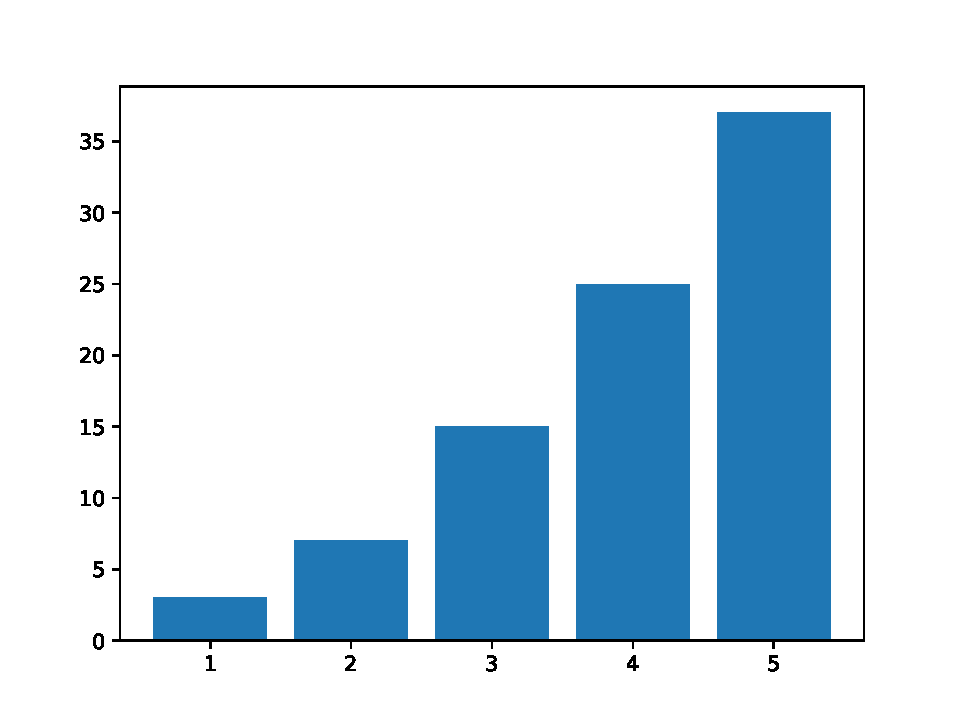
\includegraphics[scale = 0.33]{files/1.pdf}
        \centering
        \caption{Datos obtenidos.}
      \end{subfigure}
      \hspace{1.3cm}
      \begin{subfigure}[H]{0.4\textwidth}
        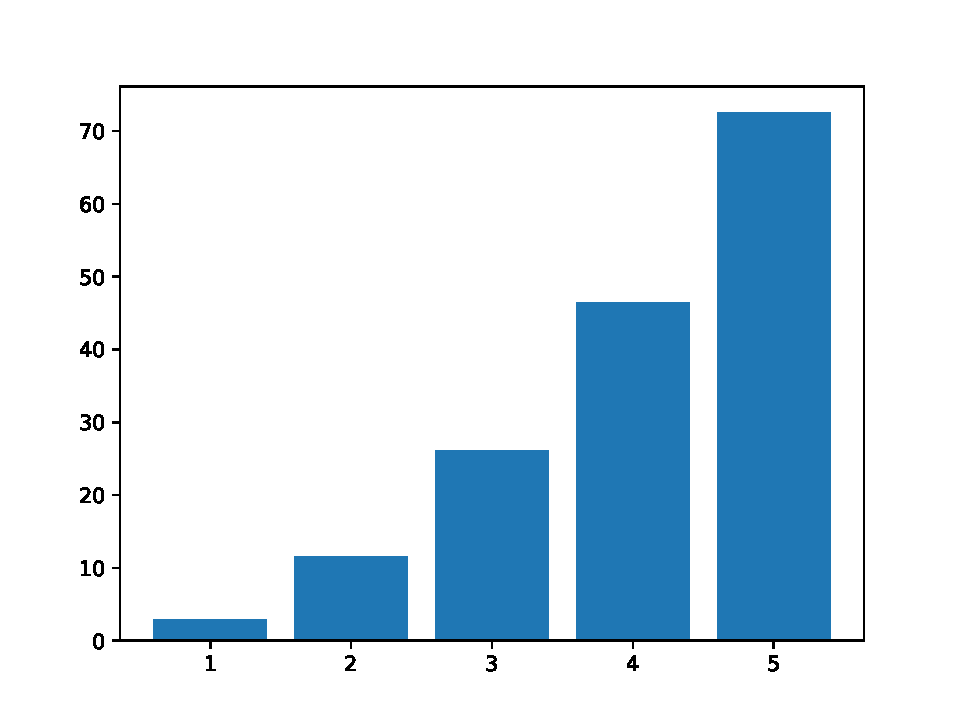
\includegraphics[scale = 0.33]{files/2.pdf}
        \centering
        \caption{Aproximación teórica.}
      \end{subfigure}
      \caption{Comparación para la función de verosimilitud.}
      \label{img:timeresults}
    \end{figure}
\end{frame}

\subsection{Modelación del Factor de Normalización}

\begin{frame}{RESULTADOS}
    \framesubtitle{Modelación del Factor de Normalización}
    \begin{itemize}
        \item Las variables aleatorias $P_t$ y $V_t$ son consideradas independientes, luego
        \begin{equation}
            P(P_t=p\wedge V_t=v)\,=\,P(P_t=p)P(V_t=v).
        \end{equation}
        \item $P_t$ y $V_t$ se distribuyen uniforme:
    \end{itemize}
    \begin{align}
        P\left( P_{t}=p \right)=&
        \begin{cases}
            \frac{1}{wh} & [[0,w]]\times[[0,h]] \\
        0 & \text{any other case}
        \end{cases}\\
        P\left( V_{t}=v \right)=&
        \begin{cases}
            \frac{1}{4} &  v\in\{(velX,0),(0,velY),(0,-velY),(-velX,0)\}\\
        0 & \text{any other case}
        \end{cases}
    \end{align}
    Donde $[[a,b]]$ representa un intervalo \textbf{discreto} entre $a,b$. Es decir
    \begin{equation*}
        [[a,b]]=\{a,\,a+1,\,a+2,...,\,b-1,\,b\},\quad a,b\in\mathbb{Z}
    \end{equation*}
\end{frame}
\subsection{Modelación de la Distribución a Priori}

\begin{frame}{RESULTADOS}
    \framesubtitle{Modelación de la Distribución a Priori}
    \begin{itemize}
        \item Como no se asumió preferencia a sectores del mapa, la variable aleatoria $N_{t+k}$ se distribuye uniforme:
        \begin{equation}
            P\left( N_{t+k}=n \right)=
            \begin{cases}
            \frac{1}{M} &  n\in[[0,M]]\\
            0 & \text{any other case}
            \end{cases}
        \end{equation}
    \end{itemize}
    Donde $M$ es el número de nodos en el panel de juego.\\
\vspace{1cm}
    \textbf{Distribución a Posteriori\\}
    Teniendo en cuenta lo planteado y la fórmula de Bayes, se tiene
    \begin{equation}
        P({ N }_{ t+k }=n\mid { P }_{ t }=p\wedge { V }_{ t}=v)=\frac{24wh(k-b)^2}{Mk(2k^2 + 3k-1)}
    \end{equation}
\end{frame}

\subsection{Grafos vs. Inferencia Bayesiana}
\begin{frame}{RESULTADOS}
    \framesubtitle{Grafos vs. Inferencia Bayesiana}
    \begin{itemize}
        \item Algoritmo más eficiente de lo esperado
        \item 25 veces para el juego original, 40 para el juego después de haber implementado el análisis bayesiano; se reportó el tiempo hasta perder.
    \end{itemize}
    \begin{table}[H]
\centering
\caption{Game time results before and after the algorithm was deployed.}
\label{tab:timeresults}
\begin{tabular}{ccc}
\hline
\textbf{Cantidad} & \textbf{Enfoque con Grafos} & \textbf{Enfoque Bayesiano} \\ \hline
\textbf{Media}     & 24.77s                   & 14.75s                      \\
\textbf{Max}      & 28.01s                   & 20.09s                      \\
\textbf{Min}      & 23.56s                   & 13.86s                     \\ \hline
\end{tabular}
\end{table}
\end{frame}

\begin{frame}{RESULTADOS}
    \framesubtitle{Grafos vs. Inferencia Bayesiana}
    \begin{figure}[H]
  \centering
  \begin{subfigure}[H]{0.4\textwidth}
    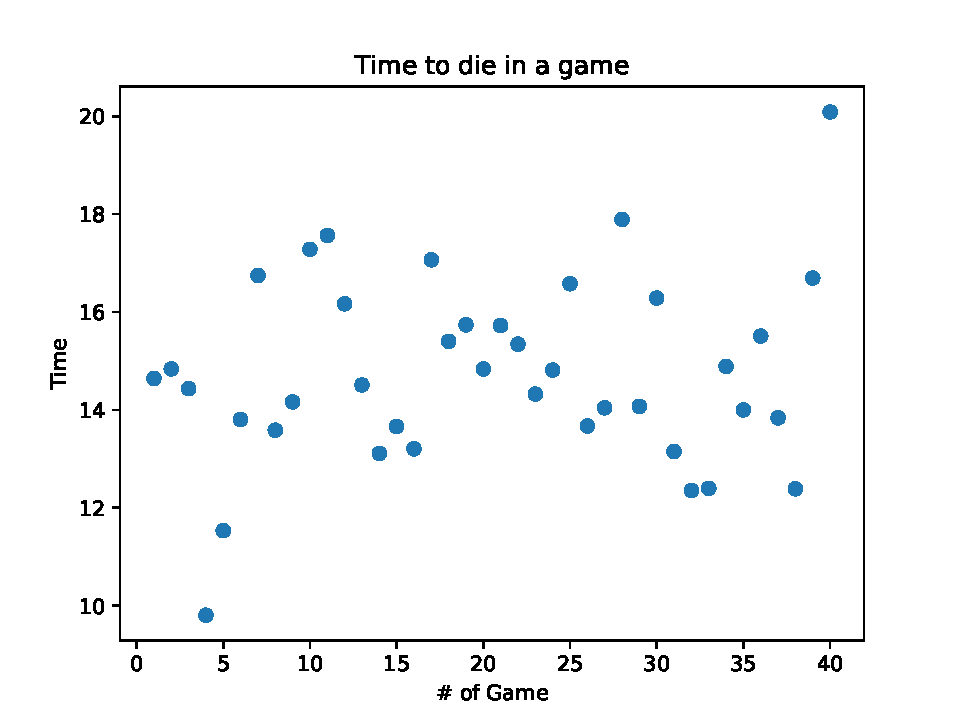
\includegraphics[scale = 0.33]{files/3.pdf}
    \centering
    \caption{Resultados utilizando grafos.}
  \end{subfigure}
  \hspace{1cm}
  \begin{subfigure}[H]{0.4\textwidth}
    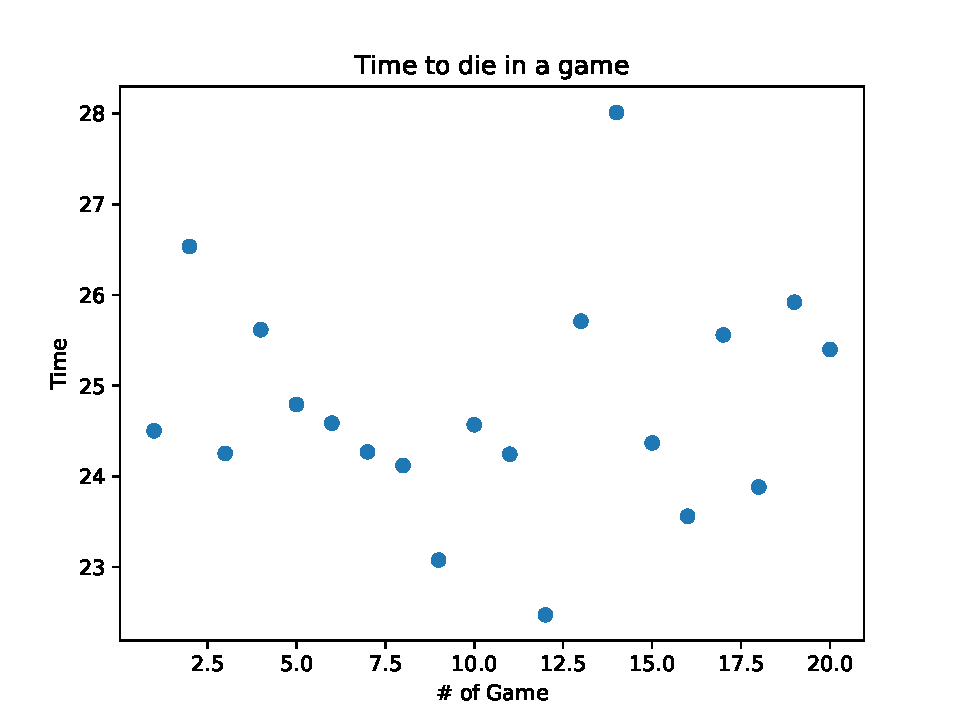
\includegraphics[scale = 0.33]{files/4.pdf}
    \centering
    \caption{Resultados utilizando inferencia bayesiana.}
  \end{subfigure}
  \caption{Resultados de tiempos hasta perder para ambos algoritmos.}
  \label{img:timeresults}
\end{figure}
\end{frame}
